% v2-acmlarge-sample.tex, dated March 6 2012
% This is a sample file for ACM large trim journals
%
% Compilation using 'acmlarge.cls' - version 1.3, Aptara Inc.
% (c) 2011 Association for Computing Machinery (ACM)
%
% Questions/Suggestions/Feedback should be addressed to => "acmtexsupport@aptaracorp.com".
% Users can also go through the FAQs available on the journal's submission webpage.
%
% Steps to compile: latex, bibtex, latex latex
%
\documentclass[prodmode,acmtap]{acmlarge}

% Metadata Information
\acmVolume{2}
\acmNumber{3}
\acmArticle{1}
\articleSeq{1}
\acmYear{2010}
\acmMonth{5}

% Copyright
%\setcopyright{acmcopyright}
%\setcopyright{acmlicensed}
%\setcopyright{rightsretained}
%\setcopyright{usgov}
%\setcopyright{usgovmixed}
%\setcopyright{cagov}
%\setcopyright{cagovmixed}

% DOI
\doi{0000001.0000001}

%ISSN
\issn{1234-56789}


% Package to generate and customize Algorithm as per ACM style
\usepackage[ruled]{algorithm2e}
\SetAlFnt{\algofont}
\SetAlCapFnt{\algofont}
\SetAlCapNameFnt{\algofont}
\SetAlCapHSkip{0pt}
\IncMargin{-\parindent}
\renewcommand{\algorithmcfname}{ALGORITHM}

% Page heads
% \markboth{D. Pineo, C. Ware and S. Fogarty}{Neural Modeling of Flow Rendering Effectiveness}

% Title portion
\title{CSE 118/218 Final Report: Team Noted}
\author{
Michael Brevard \email{A53098258} \affil{University of California, San Diego}
Dennis Kim \email{A10814282} \affil{University of California, San Diego}
Mansi Malik \email{A53096572} \affil{University of California, San Diego}
Gabe Maze-Rogers \email{A11503796} \affil{University of California, San Diego}
Thea Osinski \email{A53052464} \affil{University of California, San Diego}
Andrew Wang \email{A11262286} \affil{University of California, San Diego}
}
% NOTE! Affiliations placed here should be for the institution where the
%       BULK of the research was done. If the author has gone to a new
%       institution, before publication, the (above) affiliation should NOT be changed.
%       The authors 'current' address may be given in the "Author's addresses:" block (below).
%       So for example, Mr. Fogarty, the bulk of the research was done at UIUC, and he is
%       currently affiliated with NASA.

\begin{abstract}
TODO abstrct, actually write this
\end{abstract}


%
% The code below should be generated by the tool at
% http://dl.acm.org/ccs.cfm
% Please copy and paste the code instead of the example below.
%
% \begin{CCSXML}
% <ccs2012>
%  <concept>
%   <concept_id>10010520.10010553.10010562</concept_id>
%   <concept_desc>Computer systems organization~Embedded systems</concept_desc>
%   <concept_significance>500</concept_significance>
%  </concept>
%  <concept>
%   <concept_id>10010520.10010575.10010755</concept_id>
%   <concept_desc>Computer systems organization~Redundancy</concept_desc>
%   <concept_significance>300</concept_significance>
%  </concept>
%  <concept>
%   <concept_id>10010520.10010553.10010554</concept_id>
%   <concept_desc>Computer systems organization~Robotics</concept_desc>
%   <concept_significance>100</concept_significance>
%  </concept>
%  <concept>
%   <concept_id>10003033.10003083.10003095</concept_id>
%   <concept_desc>Networks~Network reliability</concept_desc>
%   <concept_significance>100</concept_significance>
%  </concept>
% </ccs2012>
% \end{CCSXML}

% \ccsdesc[500]{Computer systems organization~Embedded systems}
% \ccsdesc[300]{Computer systems organization~Redundancy}
% \ccsdesc{Computer systems organization~Robotics}
% \ccsdesc[100]{Networks~Network reliability}

%
% End generated code
%

% We no longer use \terms command
%\terms{Human Factors}

% \keywords{Contour perception, flow visualization, perceptual theory, visual cortex, visualization}
%
% \acmformat{Daniel Pineo, Colin Ware, and Sean Fogarty. 2010. Neural Modeling of Flow Rendering Effectiveness.}
% At a minimum you need to supply the author names, year and a title.
% IMPORTANT:
% Full first names whenever they are known, surname last, followed by a period.
% In the case of two authors, 'and' is placed between them.
% In the case of three or more authors, the serial comma is used, that is, all author names
% except the last one but including the penultimate author's name are followed by a comma,
% and then 'and' is placed before the final author's name.
% If only first and middle initials are known, then each initial
% is followed by a period and they are separated by a space.
% The remaining information (journal title, volume, article number, date, etc.) is 'auto-generated'.

\begin{document}

\maketitle

% Head 1
\section{Introduction}

In the twilight hours of World War II, Dr. Vannevar Bush singled out the inefficiency of the daunting depths of specialized information, commenting that the ability for society to leverage scientific literature is “being bogged down as [knowledge] specialization extends”. Six decades of technological revolutions later, the primary interface of sharing scientific information remains unchanged, manifesting itself as paper printouts confined to the desks of the few specialists of their respective fields. In this paper, we introduce the Noted system to make amenable the specialized texts that would be otherwise inaccessible to the general reader. Utilizing an eye-tracking sensor and gesture control armband, the Noted system bridges the knowledge gap necessary for a reader to understand a given text by unobtrusively displaying contextual annotations relevant to the content a reader is focused on. Among other design considerations, the system presents a touch-free interface that disconnects the reader from the distractions of social media to optimize the focus of the reader upon his/her text. In the following order, we shall describe the HCI and systems design considerations of the Noted system, the results of a qualitative study we conducted on the efficacy of the Noted system, our findings on the best practices in collaboration during the product development cycles of Noted, and our vision regarding future directions for information dense text interfaces.

\section{Motivation and Background}

Nature, the world’s preeminent research journal, contains over thirty separate publications - from Nature Astronomy to Nature Vaccines. Take an author contributing to one of these journals, however, chances are that any other journal may as well be written in a foreign language for that individual. Have even collegiate-level students in a typical research field read such papers, and chances are that the student encounters strenuous difficulties in comprehending the content of the texts. While it is arguable that such an outcome is an acceptable cost with respect to the fantastic academic advancements that have resulted from this specialization, one can similarly dream of the possibilities that can come of low-friction interdisciplinary collaboration of scholars of all fields, or even the inclusion of mainstream readership into the frontiers of academic thought.




In order to contribute to such a vision, we first identified the pain points associated with comprehending information dense academic texts. Based on qualitative studies that we conducted on college students exposed to academic texts, we found that the primary pain points consist of how academic papers oft assume specialized knowledge on behalf of the reader, have a tendency to make references to obscured papers that are often paywalled or otherwise inaccessible, and the difficulty of maintaining focus on the paper amidst active social media notifications. Given that the standard interface for academic papers manifests itself in a paper form that provide no means to address these pain points, readers are forced to scavenge from external resources the necessary knowledge to understand the paper, pay exorbitant fees to purchase paywalled references, or simply give up on reading the paper.




We believe that there exists tremendous potential in redesigning the interface with which users read academic texts to not only eliminate these pain points, but achieve a degree of accessibility that would allow mainstream readers to enjoy academic texts. For one, we believe that an interface for reading academic texts should bundle academic texts with an intuitive set of information necessary for its intellectual comprehension so that it is possible to “bootstrap” its comprehension. In addition, we hypothesize that such an interface should also improve comprehension of texts by controlling a reader’s attentional environment and providing a reader metacognitive feedback derived from behavioral patterns.



Such an approach is not novel in the space of general textual interfaces, however. Apple’s macOS operating system recently introduced the capability for a user to “force touch” a word in an internet browser in order to pull up the word’s definitions and origins. Amazon’s Kindle also presents a similar functionality in its interface, and found its popularity through the distraction, social-media free e-ink display it uses to display texts that demand a user’s full attention. Despite these design considerations existing in mainstream, commercial textual interfaces, existing implementations are inherently incompatible with academic texts. For one, indeterministic nature such systems utilize to contextualize textual information in non-academic papers performs extremely poorly on academic papers due to the novelty and esoteric nature of the content in academic papers. On another note, academic papers cannot be displayed in modern, text-optimized interfaces such as the Amazon Kindle due to the fact that the letter-sized papers cannot comfortably fit in the small displays of those interfaces.

\section{Design}

The Noted system is a reading interface that is tailored to augment a user’s comprehension of a given text by providing contextual information for the text’s content, creating a distraction-free environment for the user to read in, and generating metacognitive feedback for the user to analyze his own understanding of the text. To achieve this, the Noted system utilizes modern ubiquitous technology devices - notably the Eyetribe Eye Tracker in order to track the foci of a user’s attention within a textual document, and the Myo Gesture Control Armband in order to provide users a touch-free input device. Noted leverages the contextual information on the foci of the user’s attention in a textual document in order to pull up information that is relevant to the text the user is currently focusing on into a peripheral pane. For more fine-grained controls, the Noted system integrates the functionality of the Myo Gesture Control Armband so that the user can manually summon and dismiss the contextual information. As a secondary benefit, the Myo Gesture Control Armband provides a user all of the functionality necessary to control and annotate the paper the user is reading, and keeps the user away from the keyboard and mouse that a user could potentially use to respond to distractions such as social media notifications.

We built Noted with a focus on user - we adapted ourselves to look at our product in a way user would look at it. Our team member Michael’s sister Lisa is a law student and frequently juggles between reference papers. Noted aims to make her work easier by providing an interactive and comprehensive interface for reading, to allow easy effortless switching between papers.

\begin{figure}
  \centering
  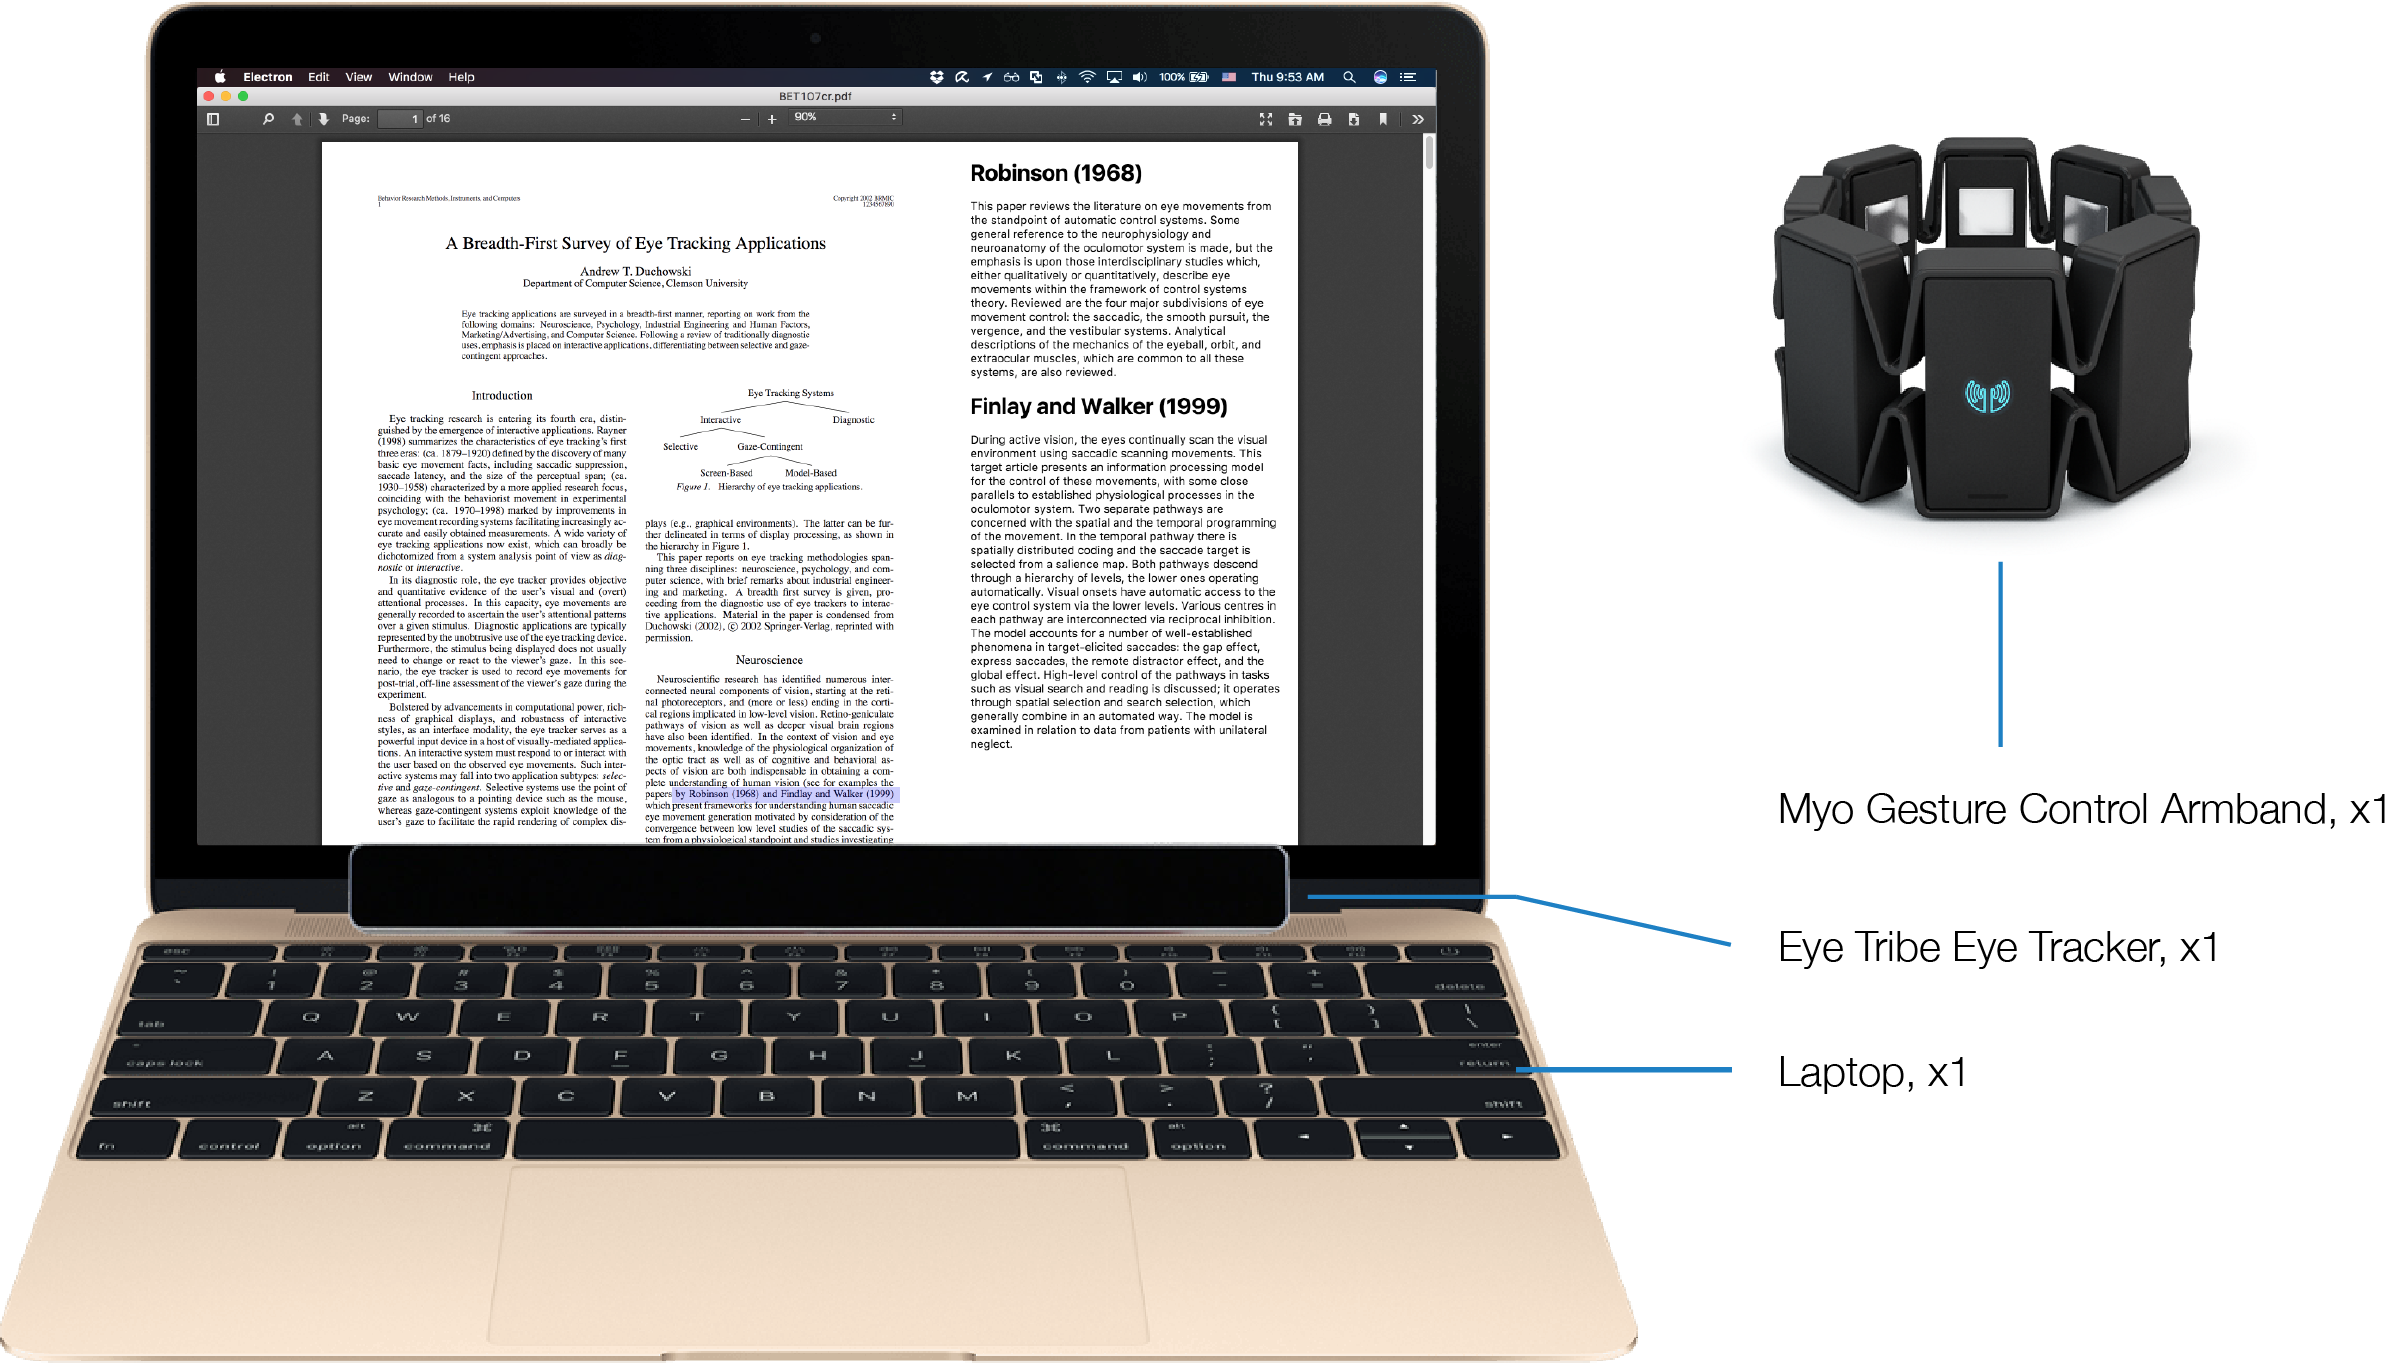
\includegraphics[width=\linewidth]{image2.png}
  \caption{Product overview of the Noted system. Supplementary information regarding the text a user is reading is displayed on the right annotation pane, and is pulled up as the user gazes upon the section of the paper that the information is relevant to.}
  \label{fig:image2}
\end{figure}

On a typical day, Lisa opens Noted and pulls up a research paper. While reading, she encounters a reference to a paper she has never read before. She flicks her hand to the right, and Noted pulls up a relevant summary of the reference paper on the right panel of the tablet.




Once she’s finished reading the summary, she can flick her hand back to the left, and the summary goes out of focus.




While reading the research paper, Lisa wants to scroll down to the next page. She looks at the bottom of the page and uses finger spread gesture to scroll down. Similarly, she can also go up by looking at the top of the page and then using the fist gesture.



On a separate note, she could choose to not close the summary, and open another summary on top of the first one, and Noted opens them up as a stack, with the recent most on top.

\begin{figure}
  \centering
  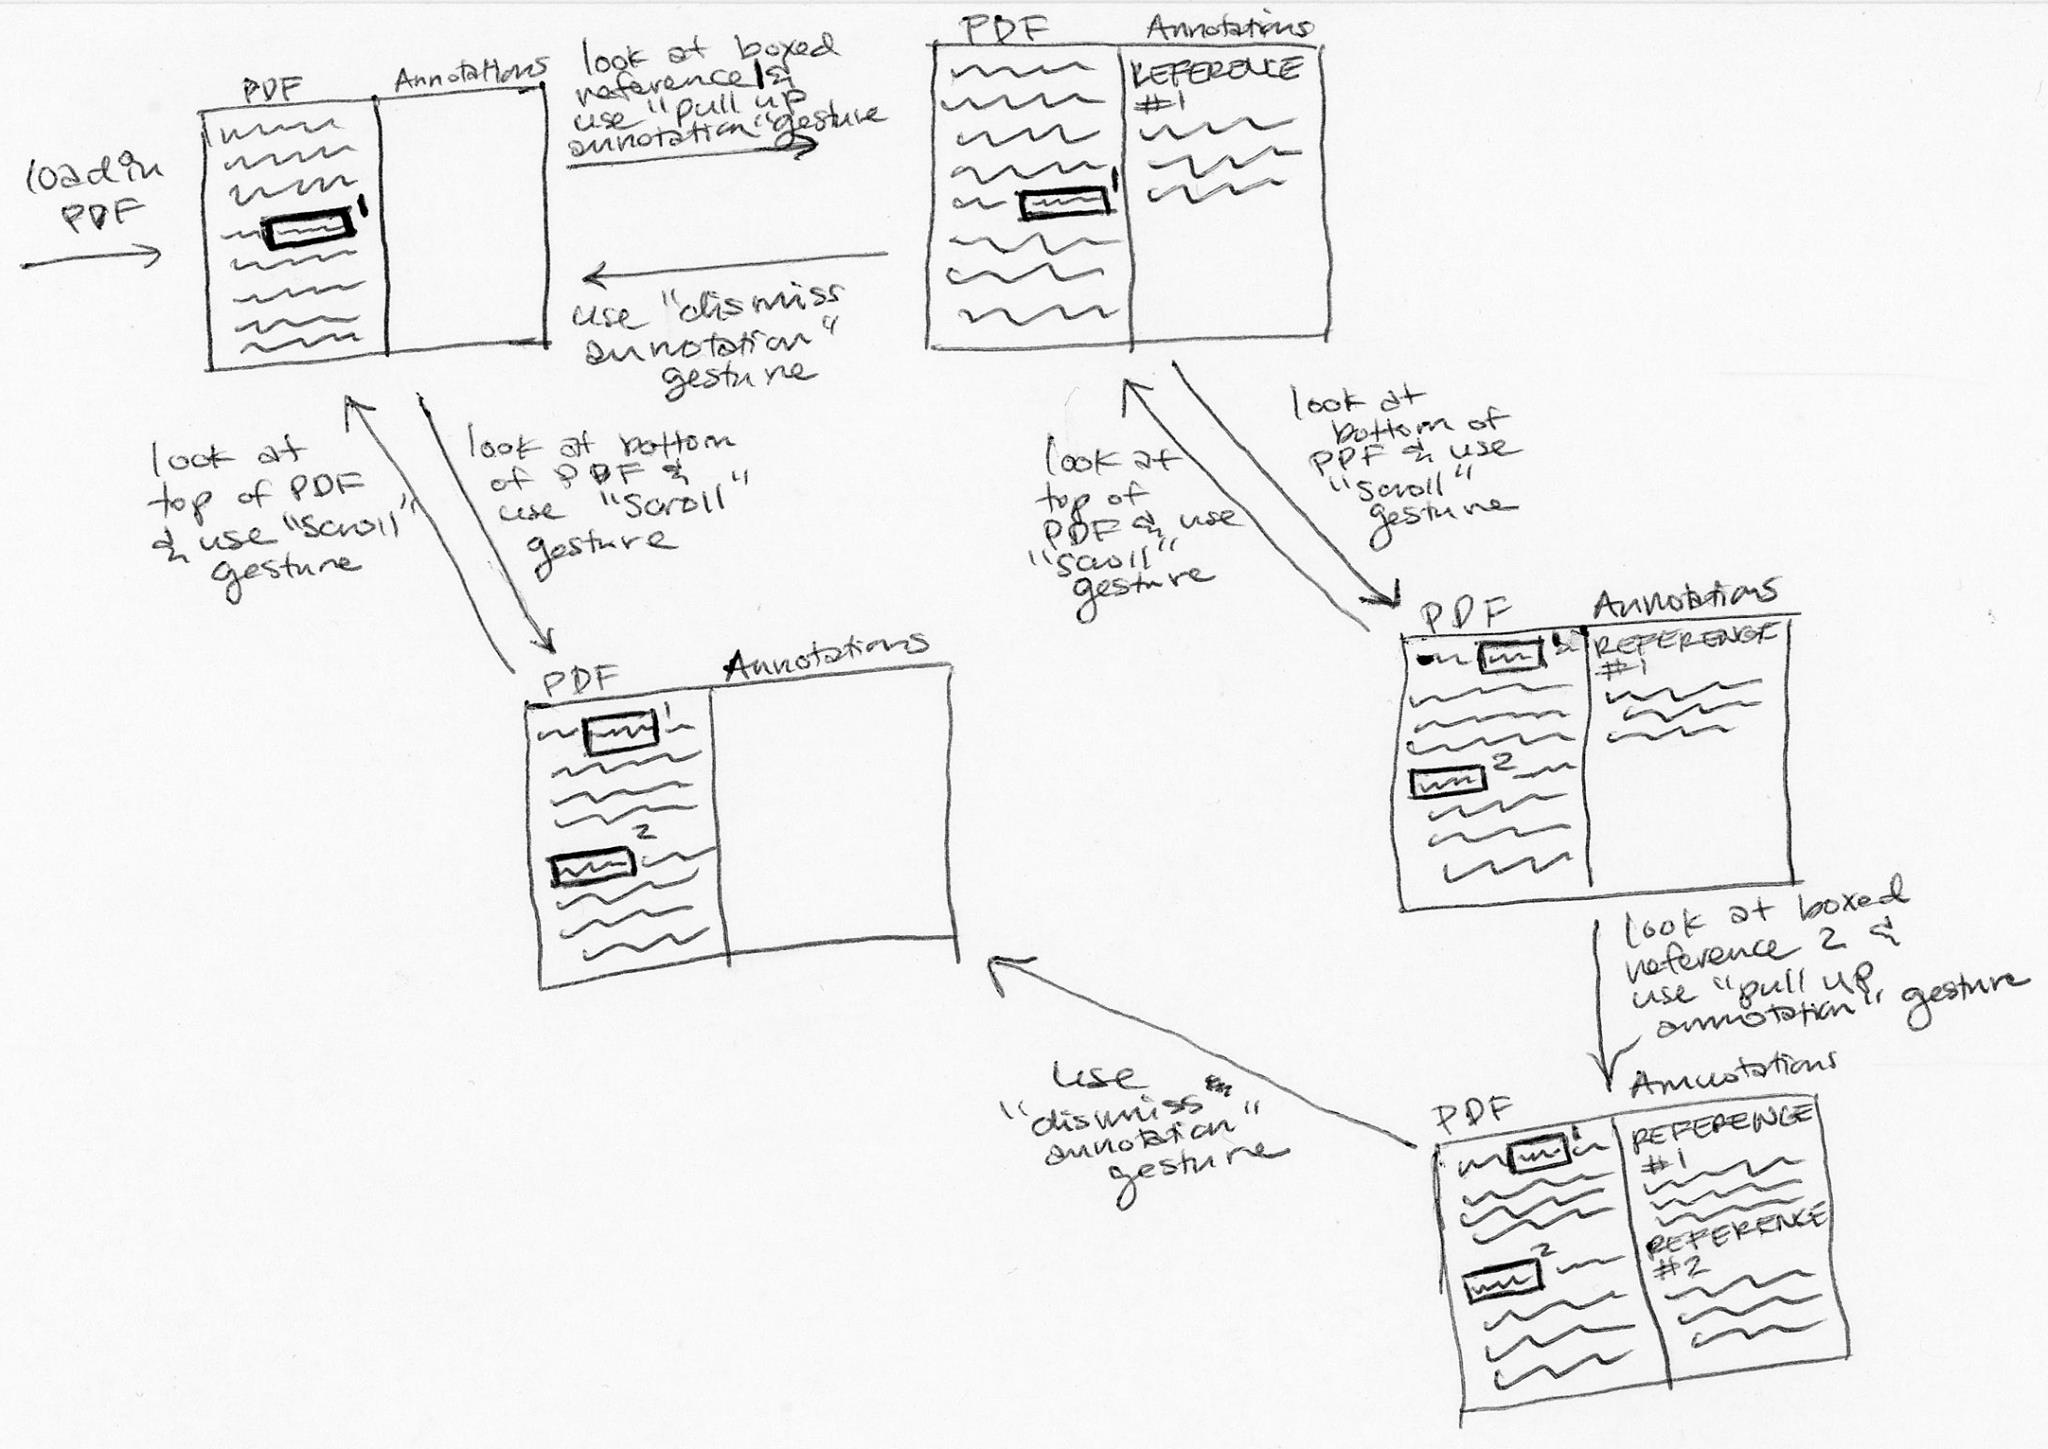
\includegraphics[width=\linewidth]{image5.png}
  \caption{Wire Frames}
  \label{fig:image5}
\end{figure}


\section{System Development}

\subsubsection{Architecture}

\begin{figure}
  \centering
  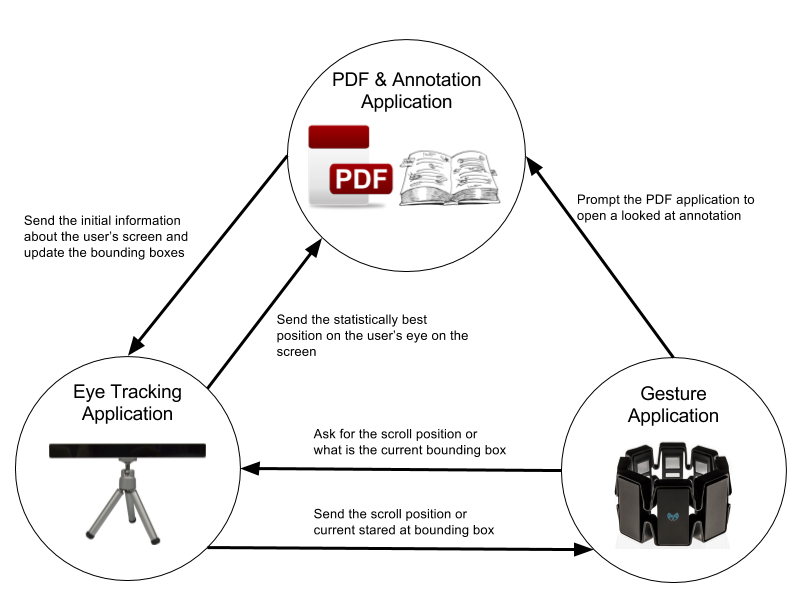
\includegraphics[scale=0.5]{image1.png}
  \caption{Architectural Design}
  \label{fig:archiecture1}
\end{figure}

The architectural design above is the high-level overview of how each application interacted with each other. The entry point of the product is through the PDF & Annotation Application which connects directly to the front-end Electron based application.


The PDF & Annotation Application is responsible for managing the user’s research papers which are in Portable Document Format (PDF) and the annotations for each PDF. This application loads the Noted Document which is the PDF with additional metadata for where the annotations are located on the document and what each annotation has for additional information. These annotation markings are referred to as bounding boxes. The bounding boxes contain a height, width, x, and y coordinate which are the size and location of the box on the document. These bounding boxes are used by the Eye Tracking Application to signal when a user is gazing at a particular annotation. There are not ubiquitous computing sensors used in the PDF & Annotation Application directly.


The input receive by the PDF & Annotation Application from the Eye Tracking Application is the current gaze point which was used for the summary feature outlined in the Features section. The current gaze point is outlined in the Eye Tracking Application. The summary section is a feature that gives a word-map of which words or phrases were gazed at by the user the most to create a visual interpretation of the document. The input received by the PDF & Annotation Application from the Gesture Application triggering the PDF & Annotation Application to load a specific annotation. The details on how the Gesture Application knows which annotation is selected is outlined in the Gesture Application section.


The output sent from the PDF & Annotation Application to the Eye Tracking Application is the initialization phase and the visible bounding boxes. The initialization phase sets the height and width of the user’s screen so the Eye Tracking Application knows the bounds on whether the user is viewing inside or outside the screen. The visible bounding boxes are used to by the Eye Tracking Application to detect the closest bounding box the user is currently gazing to. There is not output sent from the PDF & Annotation Application to the Gesture Application. The Gesture Application does not need any information from the PDF & Annotation Application, the Gesture Application feature is used to trigger the PDF & Annotation Application to trigger events.


The Eye Tracking Application is responsible for managing and analyzing the user’s eye movements. This application uses the EyeTribe Eye Tracking sensor to track the user’s eye, this also referred to as the user’s gaze. This application also performs statistically analytics to enhance the accuracy of user’s gaze which is used to detect the closest bounding box and decide the scroll or page selection. The statistically analytics that is performed to enhance the accuracy of the user’s gaze is that a history of points over a period of time is tracked. From these points, the average and standard deviation is calculated. After these calculations are completed, we detect the closest bounding box based on the average gaze and a minimum threshold for the standard deviation. The closest bounding box is decided by taking the middle point of the bounding box and finding the shortest distance from the gaze average to the closest middle point.


The panel focus is uses the input received from PDF & Annotation Application to detect whether the user is gazing at the left or right panel. This information is used by the PDF & Annotation team to detect which annotation are applicable. This information is targeted to future work that is outlined later. The initialization phase also tells the eye team the height and width of the screen which detects whether the user is looking off the screen. If the user is looking off the screen we alert the user by graying out the screen after a prolonged time of gazing off the screen.  The scroll information is used by the Gesture Application to detect whether the user wants to scroll up the document or down the document. The Eye Application detects whether the top or the bottom of the page is being looked at. The input and output of the Eye Tracking Application has been outlined above.


The Gesture Application is responsible for managing the user’s arm movement. This application uses the Myo Gesture Control sensor to track the user’s arm, this is also referred to as the user’s gesture. There are five pre-defined gestures that the user can perform with customizable gestures available which is explained in more detail in the future work section. The three main gestures that the Gesture Application captures is the swipe right, swipe left, and the finger spread gesture.


The swipe right gesture opens the annotation that is currently gazed at by Eye Tracking Application. The closest annotation is received by the Eye Tracking Application the Gesture Application triggers the PDF & Annotation Application to load the annotation that is gazed at by the user. The left swipe clears all open annotations. This feature would alert the PDF & Annotation Application to remove all currently open annotations. Lastly, the finger spread gesture triggers the PDF & Annotation Application to scroll the currently PDF document. The decision to scroll up or down is decided by the Eye Tracking Application.The input and output of the Gesture Application has been outlined above.


The main use case for Noted is the when a user looks at an annotation and swipes right to open the annotation on the right of the screen. The workflow of the problem starts at the Gesture Application. The reason that the Gesture Application is the lead application for this particular use case is because the right swipe triggers the next events. The Gesture Application captures the event of the right swipe and requests the closest annotation from the Eye Tracking Application. The Eye Tracking Application has been tracking history on the user’s gaze and calculates the closest annotation which is returned to the Gesture Application. Once this information is received from the Eye Tracking Application, The Gesture Application triggers the PDF & Annotation Application to load the annotation that is provided as input. This workflow design is that each application is modularized to handle its own particular responsibilities. From there, each section is responsible to trigger the event that takes place in its section.


Another use case for Noted is the word-cloud summary. The workflow of the problem starts the PDF & Annotation Application. The reason that the PDF & Annotation Application is the lead application for this particular use case is because they are the service that wants to generate a summary of the PDF document. The PDF & Annotation Application requests the current gaze position from the Eye Tracking Application on an interval status. The Eye Tracking Application sends the calculated gaze position to give a more enhanced gaze point. The PDF & Annotation Application uses a third party tool to generate the word-cloud based on the points provided by the Eye Tracking Application once the user is done with reading the PDF document.


TODO

\subsubsection{Technology Used}

Noted is a cross-platform desktop application. It makes use of two ubiquitous computing devices: the Myo gesture controller and the EyeTribe eye tracking device. Our implementation allows the two devices work in harmony through the user’s computer to provide a touch-free reading experience. The EyeTribe generally behaves as a pointing device, while the Myo issues commands to the system. The two devices are now discussed in more detail.


The Myo gesture controller is an armband that a Noted user will wear. It captures data relating to the user’s arm, hand, and finger movements. We use the SDK provided by Myo to facilitate the use of the device. The SDK includes all necessary components to install the Myo device drivers to a computer, a stand-alone desktop application for testing the Myo connectivity, and an API for writing scripts that recognize specific gestures. The SDK also includes several pre-programmed gestures, such as swipe left, swipe right, make a fist, and fingers spread. Because writing the scripts for new gestures requires a good deal of time to train the device to recognize the gesture, we opted to use the pre-programmed gestures in Noted where possible.


The EyeTribe eye tracker is a slim bar that sits on the computer running Noted and tracks the user’s eye position on the screen. When selecting an eye tracking device, we initially considered using the Tobii eye tracker due to its better accuracy. However, we ultimately chose the EyeTribe device due to Tobii’s poor compatibility with Mac OSX. Like the Myo, EyeTribe also comes with its own SDK. The SDK provides two desktop applications. The first detects and connects the EyeTribe, allowing it to communicate across a port. The second application provides a simple calibration interface for a connected EyeTribe device. Calibration is easy and the calibration profile will persist if the device is disconnected and reconnected later. When using Noted, it is expected that the user will connect and calibrate the EyeTribe with these SDK applications before launching Noted.


We decided that the most reasonable way to implement the Noted system would be as a desktop application. Since several of our team members had experience developing web applications, we chose to leverage this experience by building our user interface using Electron. Electron is a cross-platform framework for building a desktop application using JavaScript, HTML, or CSS. Noted has been developed using the JavaScript option. Electron has two dependencies: NodeJS and npm. As a result, Noted is built using both as well.


There are many existing useful packages available via npm and Noted uses several. First, our user interface is built using a PDF viewer npm package. This package allows us to easily load in and display the PDF document in the left panel. Second, both Myo and EyeTribe require listeners to pull data from their connected ports. Fortunately, npm packages already exist for both devices. Noted makes use of these packages when creating the Myo and EyeTribe listeners. Finally, we also make use of a wordcloud package to provide the user with a report of the words in the document that the user spent the most time gazing at while reading the document. This is discussed in more detail in the Features section.

\subsubsection{Features}

Our Noted prototype provides a complete, hands-free reading environment for PDF documents. With the prototype, the user may load in a document with annotated references, scroll through the document, and pull up or dismiss any of the annotated references. In this section, we go into each of these features in more detail.


The first step when operating Noted is to load in a PDF with annotated references. Upon launching, the Noted prototype loads in an example PDF document, in this case a technical research paper, and uses the PDF viewer to display the document in the lefthand panel of the Noted interface. The right hand panel, where annotations will be loaded, is initially blank. The PDF in the left panel is further enhanced by drawing visible bounding boxes around any annotated references. Each bounding box is linked to the specific annotation for that reference. In a final version of the product, this document would be created by a publisher. For our prototype, we have manually placed these bounding boxes and written the corresponding annotations. Because the prototype uses a general PDF viewer, any PDF with or without annotations can be loaded into Noted. Should the user have a PDF document that lacks annotations, he or she can still load this PDF to enjoy a hands-free reading experience.


Upon launch, both Myo and the EyeTribe eye tracker must be connected and calibrated beforehand via their normal processes. Listeners are established to pull data from the Myo and EyeTribe ports as the user progresses through the document. These data are pulled in a continuous stream. In order to reduce inaccuracy with the EyeTribe data, coordinates corresponding to the last second of the user’s gaze history are stored by the application.


The user is now free to read the document normally. To facilitate a hands-free experience, the user is able to perform scrolling actions without relying on a mouse. The user need only look toward the top or the bottom of the document and perform the “scroll” gesture. The Myo detects this gesture and sends a query to the Noted front-end. The front-end in turn issues a query to the EyeTribe requesting which direction to scroll. The EyeTribe detects whether the user is looking toward the top or bottom and responds accordingly. Using this response, the front-end is able to scroll the document in the direction of the user’s gaze. The entire process is quick and seamless, allowing the user to easily scroll through the document using only the Noted devices.


Noted’s major feature is the ability for the user to bring up annotations for references within the document. As mentioned above, an annotated PDF features visible bounding boxes around the corresponding references. As the user reads, the user may gaze at one of these bounding boxes. While looking at the bounding box, the user performs the “pull up annotation” gesture. Once again, the Myo signals to the front-end that the user wishes to perform an operation, this time opening a reference annotation. The front-end sends a message to the EyeTribe requesting the reference number for the bounding box upon which the user is gazing. As part of this request, the front-end passes along a list of all the currently visible bounding boxes and their locations on the screen.


The detection logic begins by computing the average coordinate from the gaze history. It also computes the standard deviation of this gaze history in order to provide a level of confidence in the detection. Detection happens in two stages. First, the coordinate is compared against the list of visible bounding boxes to determine if the coordinate falls within a bounding box. Because of the inaccuracy in the EyeTribe data and the size of the bounding boxes, the coordinate does not always fall within the bounding box but may be nearby instead. For this reason, if the first stage fails, a second stage initiates that computes the distance from the coordinate to the center of each bounding box. The bounding box at the shortest distance from the coordinate is then chosen as the detected bounding box.


After success in either stage, the number of the detected bounding box is returned to the front-end. The front-end may then retrieve the annotation corresponding to the detected bounding box and display it in the righthand panel. If the righthand panel is not empty, the new annotation is simply added below any existing annotations. The annotations will persist in the panel until the user dismisses them.


In order to dismiss annotations, the user first issues a “dismiss annotations” gesture. Myo detects and recognizes this gesture and sends the appropriate command to the front-end. The front-end then clears the annotations currently present in the righthand panel. If there is more than one annotation, it clears all of them, leaving the panel blank once more.


As the user reads, the EyeTribe also sends the current gaze coordinate to the front-end. The front-end uses this data to determine which word the user is gazing at and records how long the user spends on this word. Once the user has finished the document, he or she is able to pull up a gaze summary of where the most time was spent in the document. The front-end makes use of the wordcloud package mentioned earlier to report this data to the user. This allows the user to reflect on which sections of the document required the most attention, and possibly return to these sections in the future for further study.


\section{Testing and Evaluation}

\subsubsection{Testing Methodology}
Our means of testing adopted the agile methods where we would meet up every week to get together with our respected group and the whole team to talk about further development and current issues. During the meeting with our respected groups, we would unit test each technology to see the success of each functionality. When week 7 came along, we devoted more time with testing the application as a group so that we can integrate the different technologies to the front-end. Another testing methodology that we used when we integrated the technologies was scenario based testing where we simulated different use cases to help us think of more user-friendly features and to be able to test the fluidity of those functionalities. For example, to enhance the scrolling functionality we had visioned how the eye-tracking system can tell if the user is looking at the top half of the screen and from there the user to use one of the gestures to scroll up; and vice versa.  The main way we were testing these scenarios was by using the testing tool in Electron that incorporated the built in webkit engine.

\begin{figure}
  \centering
  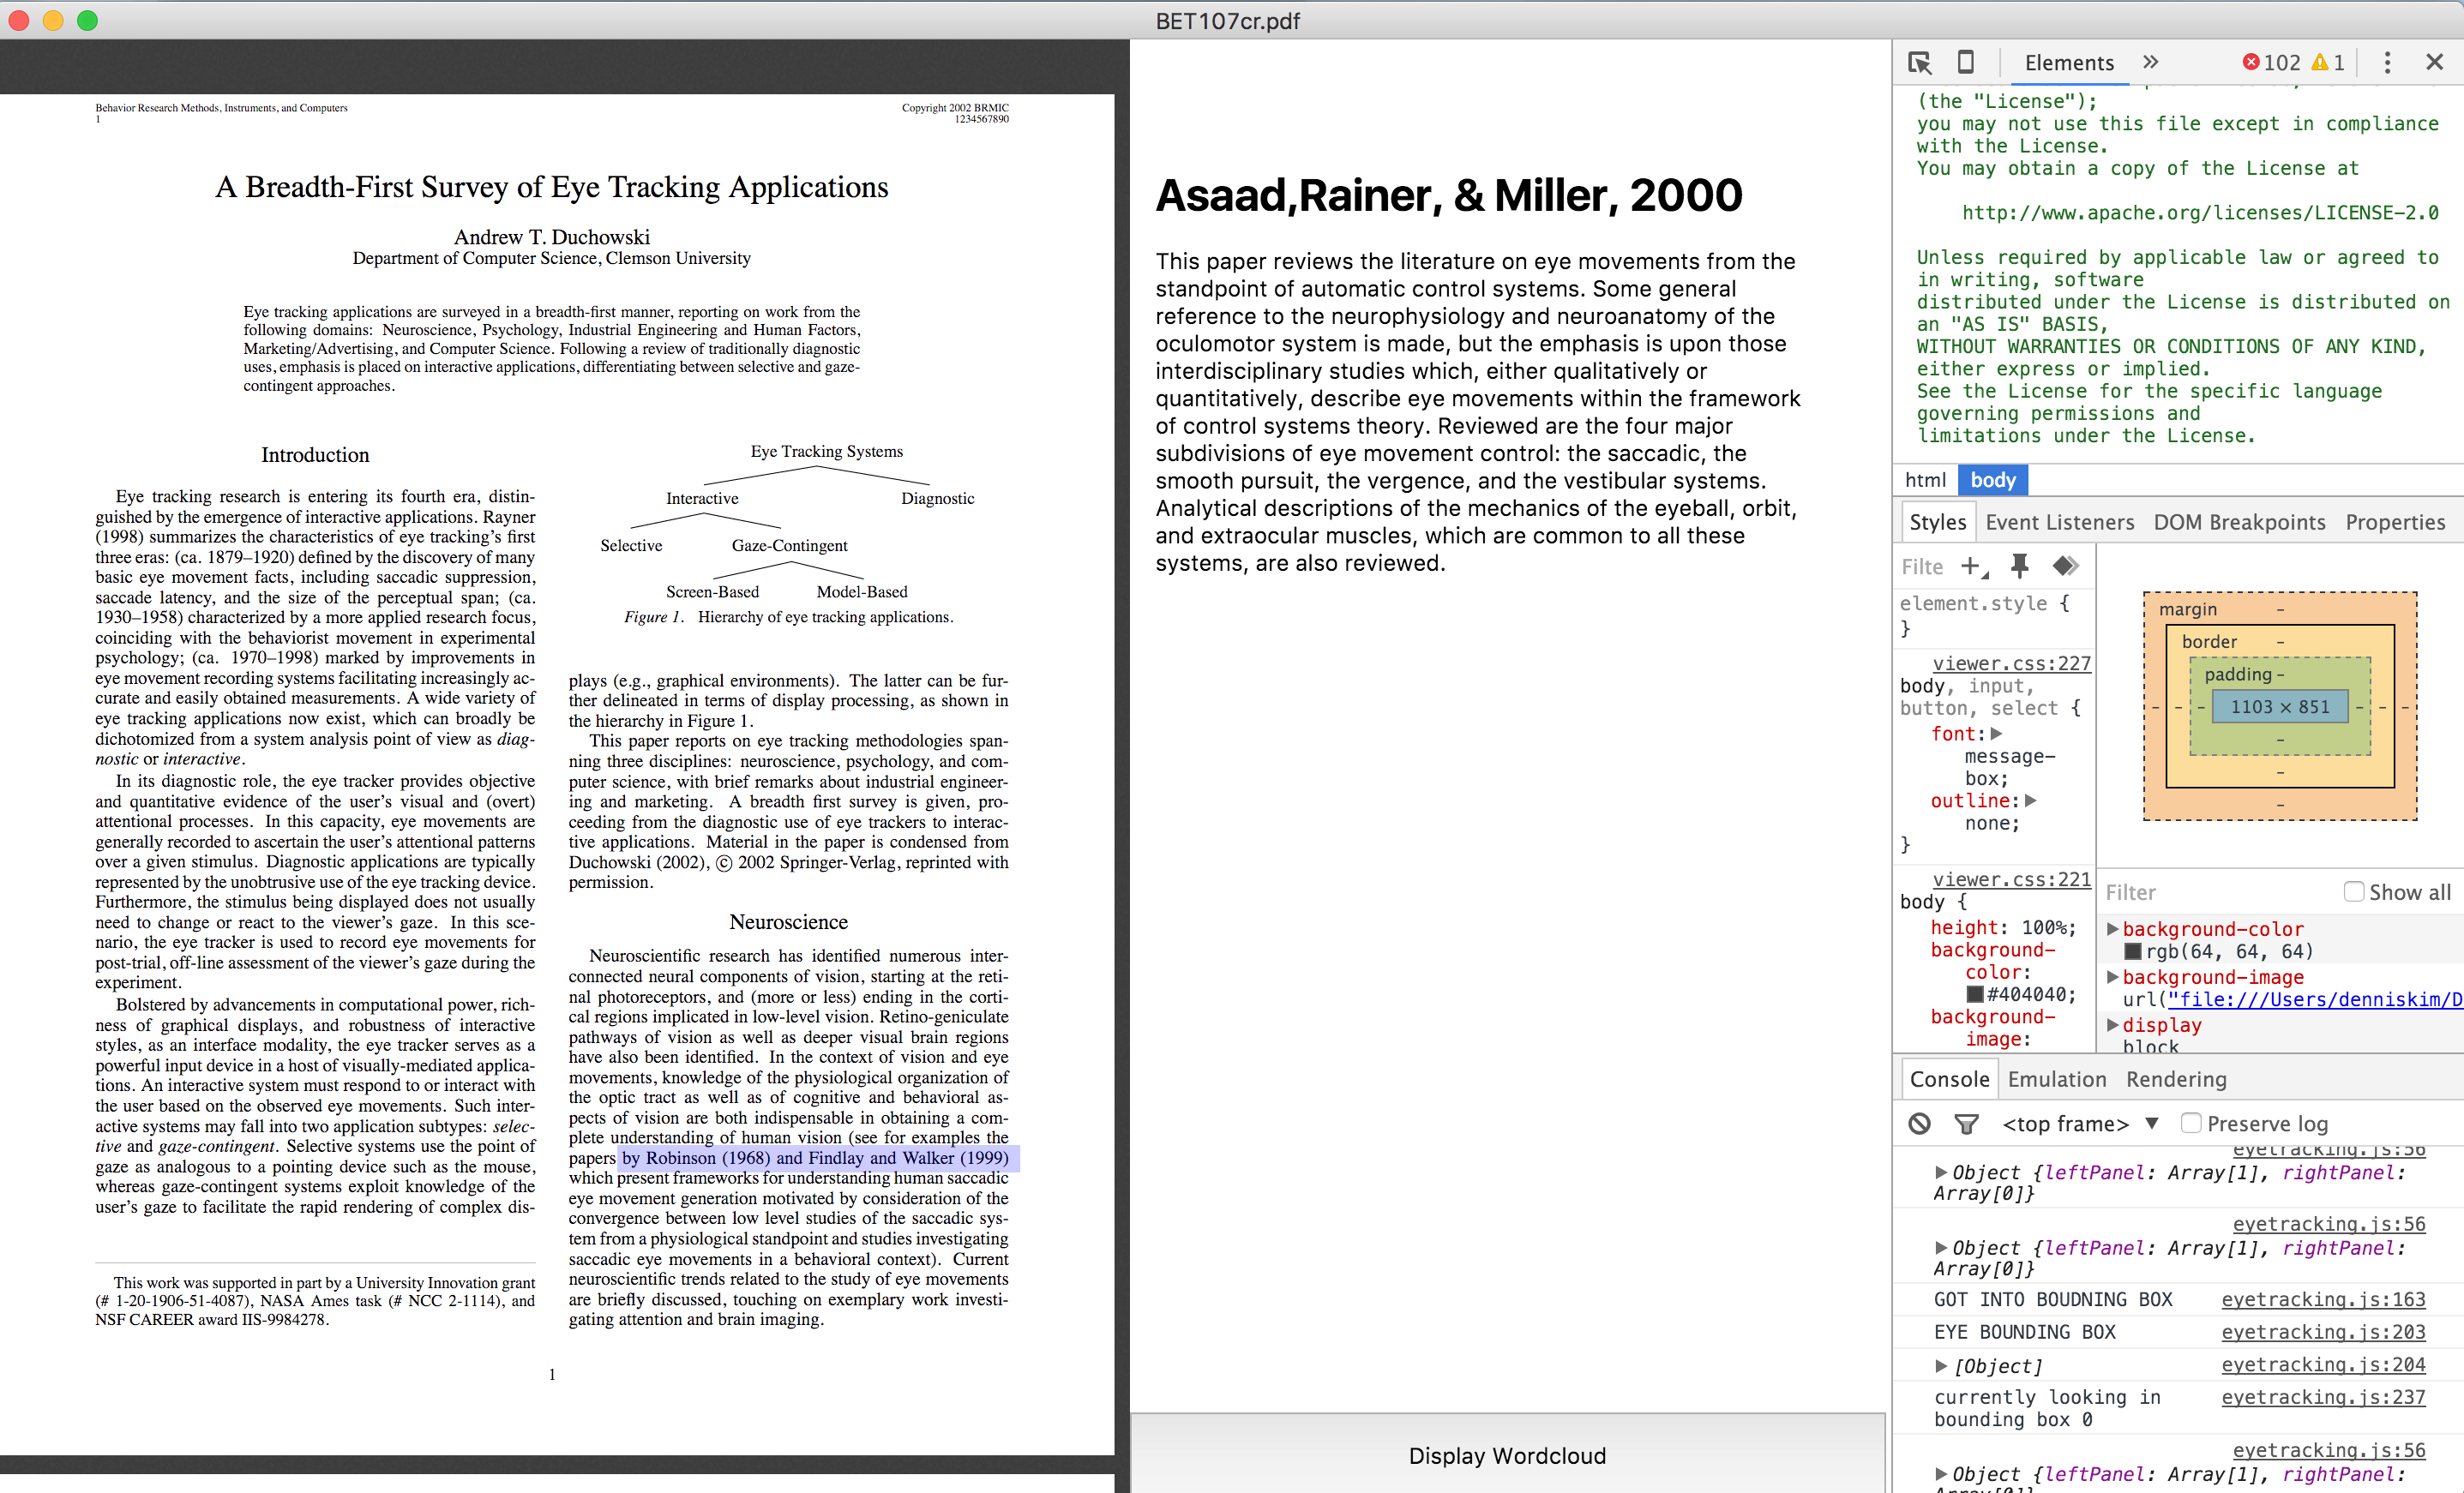
\includegraphics[scale=0.2]{image7.png}
  \caption{This is the Electron application. On right is the testing tool that was used.}
  \label{fig:image7}
\end{figure}

\subsubsection{Progression and Adapation}
Throughout the development and progression of our project, we had stayed consistent to the motivation of why we initially started our project. Our initial motivation for Noted was to create a more fluid and simple way of reading a dense research paper with a lot of supplementary information from external resources, where we can create a distraction free environment for users by dismissing the keyboard and mouse. We were able to withhold our identity and create an application where users are able to have all the available resources at the tip of their fingertips; and also are able to control everything using their eyes and hand gestures, creating a distraction free medium of studying.
However due to time constraint, we were not able to get to some of the features that we had envisioned to enhance the user’s experience even more. Those features includes the power to annotate the document and the feature that would allow publishers to submit their papers into our back-end server.

\begin{figure}
  \centering
  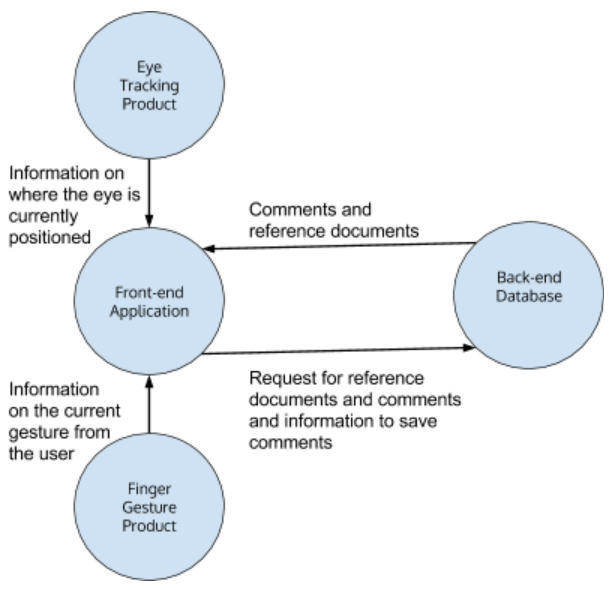
\includegraphics[scale=0.6]{image6.png}
  \caption{Our initial system architecture and goal }
  \label{fig:image6}
\end{figure}


\section{Collaboration}

\subsubsection{Team Structure}
The way we structured our team was to divide into three groups of two, where each group focused on a specific task/technology: Front-end, EyeTracking, and Myo team. Initially thinking that we make faster progress, we had envisioned that the Myo team would branch out into the backend development; however, due to the lack of time, we were not able to set up a back-end for our application. To assign people into groups, we asked a set of questions: such as personal preference on what technology one would like to work with and people’s strength. With that we had assigned Gabe and Andrew onto the front-end team, Michael and Thea onto the EyeTracking team, and Mansi and Dennis onto the Myo team.

\subsubsection{Contributions}
The front-end team was able to find an open source PDF renderer application in Electron; and made appropriate changes and implementations to tailor our project. More specifically, Andrew and Gabe developed the Bounding Box feature that created bounding box around different resources that are incorporated in the research paper. Another feature that Andrew and Gabe developed was the creation of a side pane that would render the content of the different resources. They also created an algorithm that was inherited from an open source library to find the unigram probability where we can use that to summarize the user’s most looked section. Lastly, Andrew was the one who created the Noted web page.

As for the eye-tracking team, Michael and Thea were able to set up a framework for the EyeTribe onto the front-end application. Using this schema Michael and Thea were able to successfully grab the data from the EyeTribe instance. With that they implemented the gaze history feature that …. Other features that they worked on was to check if the user was looking at a bounding box, or to grab the closest bounding box in the proximity of the coordinates of the EyeTribe instance…

As for the Myo team, Dennis and Mansi were able to set up and create a framework to connect to the front-end using a open source web daemon. With that, we implemented different features that listened for different gesture events. Most of the features were implemented by the other team where we were mainly tasked to integrate them to create a fluid experience for the user. Given the features from the front-end team and eye-tracking team, such as scrolling, opening up the pane, and getting the coordinates for the closest bounding box, Dennis and Mansi integrated these into different gesture events.

As for the non-technical work, such as the weekly updates, each team were responsible for updating the deliverables per week and elaborate on what needs to be done next week. Also for the midterm presentations, we were able to work on the presentations together when we met as a team every Thursday. Lastly the scrum report was handled by the graduate student, in which they  they switched off the responsibility every week.

The plans for our final report was to divide it into groups, where we allocated less work for the group that was responsible for more of the coding or had more features to develop, specifically the front-end team. Andrew and Gabe were responsible for the Executive Summary, Introduction, and the Conclusion/ Future work. Mansi was responsible for Motivation & Background, Design (where we used Thea’s wireframes), and Dennis was responsible for the Testing/Evaluation and the Collaboration section. And Michael and Thea were responsible for the System Development section.

\begin{figure}
  \centering
  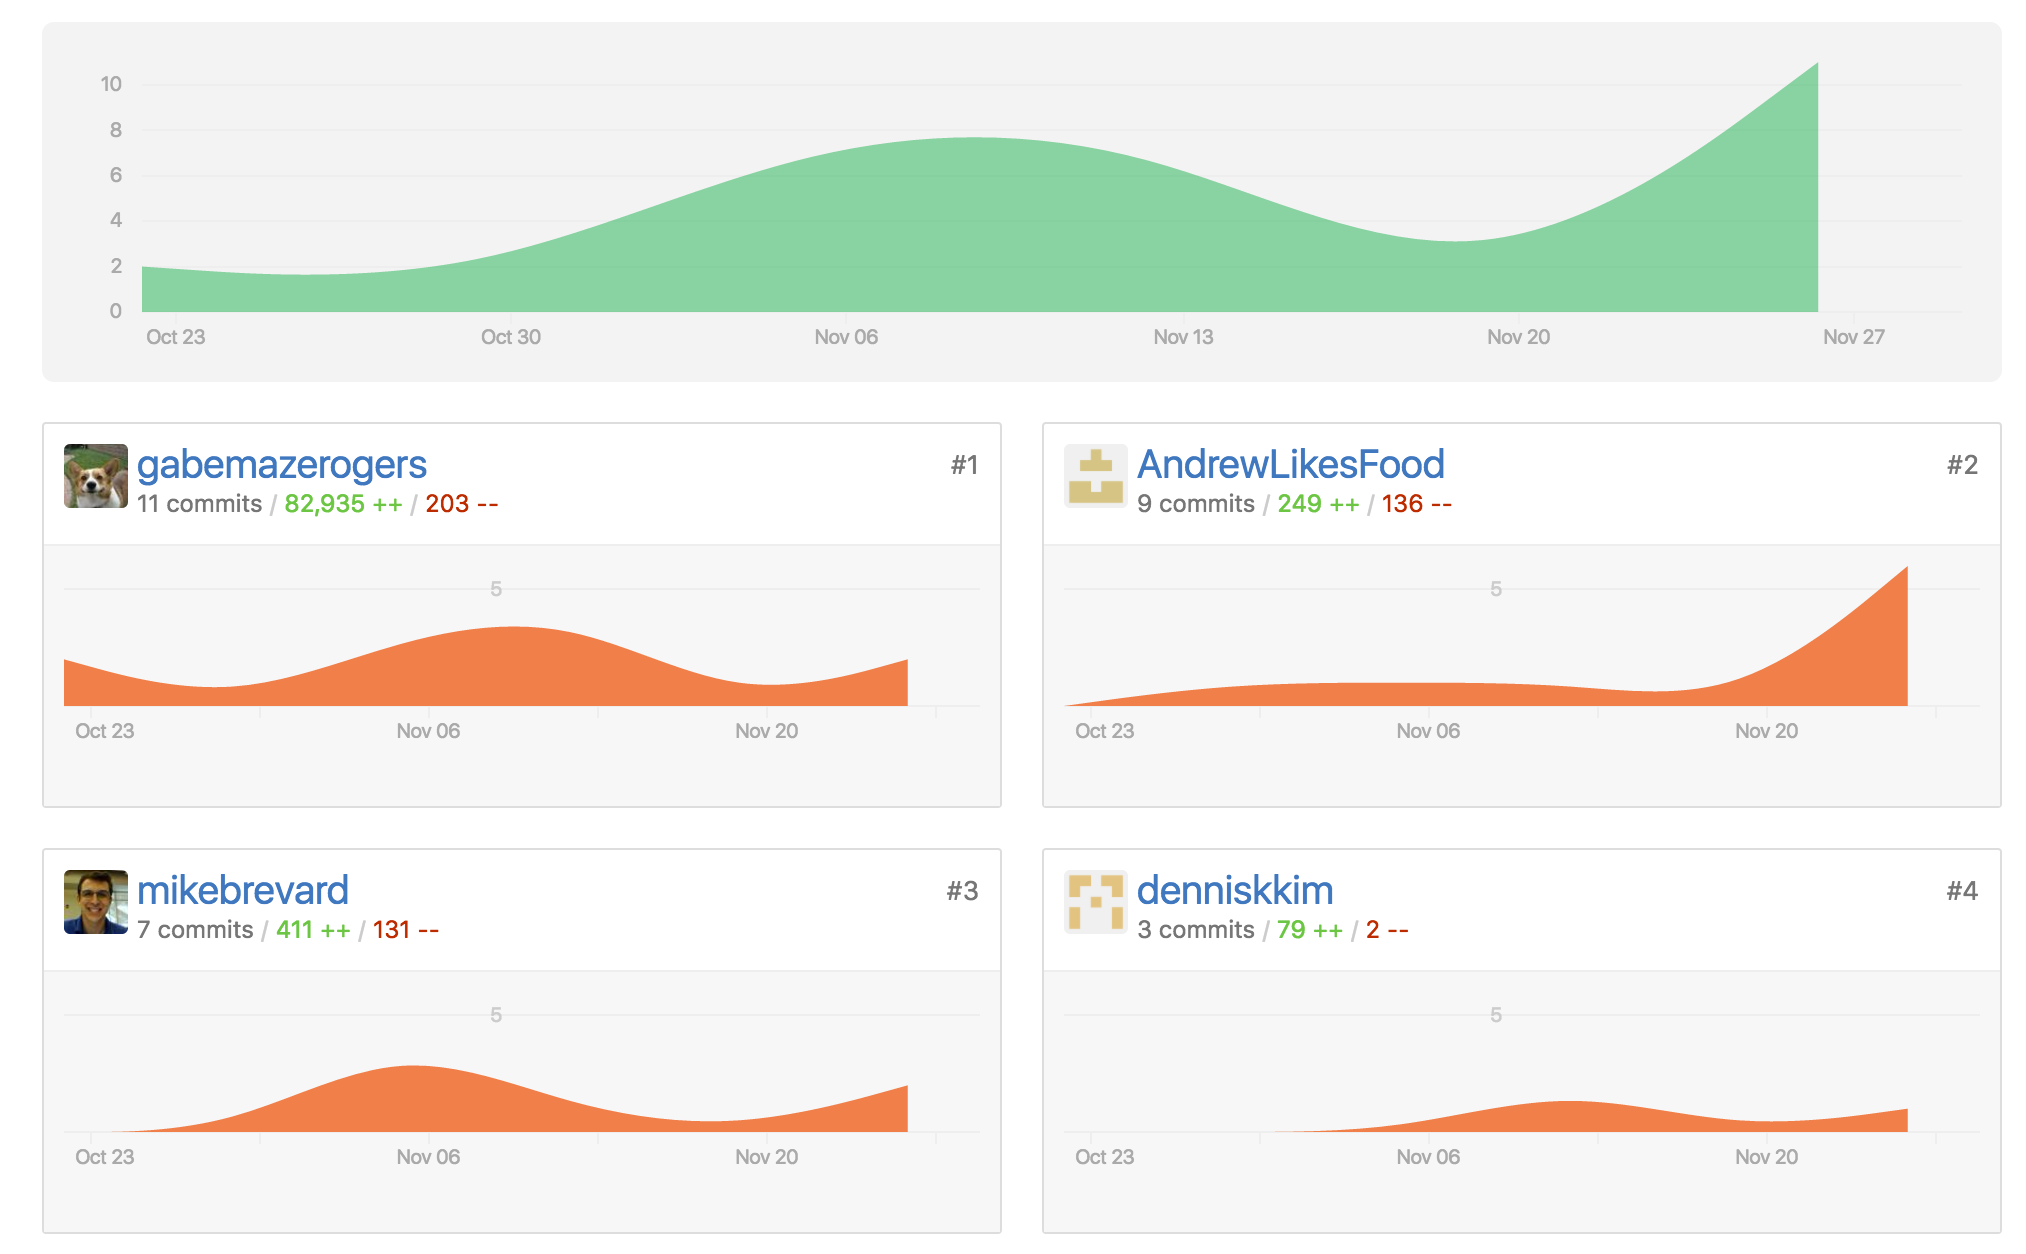
\includegraphics[scale=0.4]{image3.png}
  \caption{GitHub Commit History (Thea and Michael, Dennis and Mansi pair programmed)}
  \label{fig:image3}
\end{figure}

\subsubsection{Organizational Tools/Weekly Meetings}
To make sure that we were having good progress, we had set Thursdays from 11 AM to 1 PM as our meeting times where we discussed what to do next week and discuss the project as a whole. During this meeting time, we also collaborated on the two presentations. Starting week 8, we had decided to have a hackathon once a week from then to the end of week 10, just to solidify all our features and integrate each side of the project. Our main collaborating tool was using Slack, where we set up channels for each respected team. Some issues that we had with Slack during the first two weeks were that people were not checking their Slack as frequently and we addressed the issue by keeping the notifications on and downloading the application onto our phones.

\begin{figure}
  \centering
  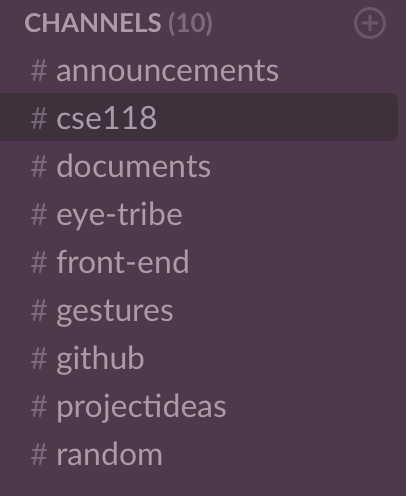
\includegraphics[scale=0.5]{image4.png}
  \caption{Slack groups and how we organized our communication}
  \label{fig:image4}
\end{figure}

\subsubsection{Problems and Issue Resolution}



\section{Conclusion and Future Work}

\subsubsection{Future Work}

This past quarter, our team has designed and developed a solid infrastructure for the Noted system to handle PDFs with supplementary metadata.  To improve this infrastructure in the future, we want to focus on improving the publisher’s ability to provide metadata to augment the papers. The Noted platform would ideally support interactive modules to video lectures or even 3D animations. Currently, Noted’s main limiting factor is the physical technology required, which is something that must be improved for its spread and adoption. For the majority of the population using multiple physical devices with their personal computer to have an enhanced reading experience is not practical. In addition, the devices we used for Noted, the EyeTribe and Myo, are usable for demonstrations and testing but their capabilities and fidelity are both too limited for widespread use. We need to focus on improve existing technologies, such as personal computers, to provide the benefits of eye and gesture trackers without requiring separate devices.

\subsubsection{Conclusion}

Marcia Riley of the Georgia Institute of Technology describes the purpose of Ubiquitous Computing as a “paradigm shift where technology becomes virtually invisible in our lives”. With Noted, our team interpreted this as using technology to augment our daily lives without creating any additional roadblocks. With the current state of eye and gesture tracking technology this is difficult due to technological limitations, but Noted serves a proof of concept of what the future of interacting with literature can be. Noted seamlessly integrates eye and gesture tracking technologies to address issues that have plagued a medium that has existed for centuries. Recent innovations to how we consume literature have been made with the proliferation of portable computing devices and digital media, but little has been done to take full advantage of the possibilities of literature as a digital medium. Noted integrates ubiquitous computing devices to provide readers of academic papers and general literature a greater breadth of knowledge by combining the physical and virtual environment to seamlessly to create a distraction free learning environment.


% Appendix
\appendix
\section*{APPENDIX}
\setcounter{section}{1}

% Bibliography
\bibliographystyle{ACM-Reference-Format-Journals}
\bibliography{acmlarge-sample-bibfile}
TODO
                                % Sample .bib file with references that match those in
                                % the 'Specifications Document (V1.5)' as well containing
                                % 'legacy' bibs and bibs with 'alternate codings'.
                                % Gerry Murray - March 2012

\elecappendix


\end{document}
% End of v2-acmlarge-sample.tex (March 2012) - Gerry Murray, ACM
